% Options for packages loaded elsewhere
\PassOptionsToPackage{unicode}{hyperref}
\PassOptionsToPackage{hyphens}{url}
%
\documentclass[
]{article}
\usepackage{amsmath,amssymb}
\usepackage{iftex}
\ifPDFTeX
  \usepackage[T1]{fontenc}
  \usepackage[utf8]{inputenc}
  \usepackage{textcomp} % provide euro and other symbols
\else % if luatex or xetex
  \usepackage{unicode-math} % this also loads fontspec
  \defaultfontfeatures{Scale=MatchLowercase}
  \defaultfontfeatures[\rmfamily]{Ligatures=TeX,Scale=1}
\fi
\usepackage{lmodern}
\ifPDFTeX\else
  % xetex/luatex font selection
\fi
% Use upquote if available, for straight quotes in verbatim environments
\IfFileExists{upquote.sty}{\usepackage{upquote}}{}
\IfFileExists{microtype.sty}{% use microtype if available
  \usepackage[]{microtype}
  \UseMicrotypeSet[protrusion]{basicmath} % disable protrusion for tt fonts
}{}
\makeatletter
\@ifundefined{KOMAClassName}{% if non-KOMA class
  \IfFileExists{parskip.sty}{%
    \usepackage{parskip}
  }{% else
    \setlength{\parindent}{0pt}
    \setlength{\parskip}{6pt plus 2pt minus 1pt}}
}{% if KOMA class
  \KOMAoptions{parskip=half}}
\makeatother
\usepackage{xcolor}
\usepackage[margin=1in]{geometry}
\usepackage{color}
\usepackage{fancyvrb}
\newcommand{\VerbBar}{|}
\newcommand{\VERB}{\Verb[commandchars=\\\{\}]}
\DefineVerbatimEnvironment{Highlighting}{Verbatim}{commandchars=\\\{\}}
% Add ',fontsize=\small' for more characters per line
\usepackage{framed}
\definecolor{shadecolor}{RGB}{248,248,248}
\newenvironment{Shaded}{\begin{snugshade}}{\end{snugshade}}
\newcommand{\AlertTok}[1]{\textcolor[rgb]{0.94,0.16,0.16}{#1}}
\newcommand{\AnnotationTok}[1]{\textcolor[rgb]{0.56,0.35,0.01}{\textbf{\textit{#1}}}}
\newcommand{\AttributeTok}[1]{\textcolor[rgb]{0.13,0.29,0.53}{#1}}
\newcommand{\BaseNTok}[1]{\textcolor[rgb]{0.00,0.00,0.81}{#1}}
\newcommand{\BuiltInTok}[1]{#1}
\newcommand{\CharTok}[1]{\textcolor[rgb]{0.31,0.60,0.02}{#1}}
\newcommand{\CommentTok}[1]{\textcolor[rgb]{0.56,0.35,0.01}{\textit{#1}}}
\newcommand{\CommentVarTok}[1]{\textcolor[rgb]{0.56,0.35,0.01}{\textbf{\textit{#1}}}}
\newcommand{\ConstantTok}[1]{\textcolor[rgb]{0.56,0.35,0.01}{#1}}
\newcommand{\ControlFlowTok}[1]{\textcolor[rgb]{0.13,0.29,0.53}{\textbf{#1}}}
\newcommand{\DataTypeTok}[1]{\textcolor[rgb]{0.13,0.29,0.53}{#1}}
\newcommand{\DecValTok}[1]{\textcolor[rgb]{0.00,0.00,0.81}{#1}}
\newcommand{\DocumentationTok}[1]{\textcolor[rgb]{0.56,0.35,0.01}{\textbf{\textit{#1}}}}
\newcommand{\ErrorTok}[1]{\textcolor[rgb]{0.64,0.00,0.00}{\textbf{#1}}}
\newcommand{\ExtensionTok}[1]{#1}
\newcommand{\FloatTok}[1]{\textcolor[rgb]{0.00,0.00,0.81}{#1}}
\newcommand{\FunctionTok}[1]{\textcolor[rgb]{0.13,0.29,0.53}{\textbf{#1}}}
\newcommand{\ImportTok}[1]{#1}
\newcommand{\InformationTok}[1]{\textcolor[rgb]{0.56,0.35,0.01}{\textbf{\textit{#1}}}}
\newcommand{\KeywordTok}[1]{\textcolor[rgb]{0.13,0.29,0.53}{\textbf{#1}}}
\newcommand{\NormalTok}[1]{#1}
\newcommand{\OperatorTok}[1]{\textcolor[rgb]{0.81,0.36,0.00}{\textbf{#1}}}
\newcommand{\OtherTok}[1]{\textcolor[rgb]{0.56,0.35,0.01}{#1}}
\newcommand{\PreprocessorTok}[1]{\textcolor[rgb]{0.56,0.35,0.01}{\textit{#1}}}
\newcommand{\RegionMarkerTok}[1]{#1}
\newcommand{\SpecialCharTok}[1]{\textcolor[rgb]{0.81,0.36,0.00}{\textbf{#1}}}
\newcommand{\SpecialStringTok}[1]{\textcolor[rgb]{0.31,0.60,0.02}{#1}}
\newcommand{\StringTok}[1]{\textcolor[rgb]{0.31,0.60,0.02}{#1}}
\newcommand{\VariableTok}[1]{\textcolor[rgb]{0.00,0.00,0.00}{#1}}
\newcommand{\VerbatimStringTok}[1]{\textcolor[rgb]{0.31,0.60,0.02}{#1}}
\newcommand{\WarningTok}[1]{\textcolor[rgb]{0.56,0.35,0.01}{\textbf{\textit{#1}}}}
\usepackage{graphicx}
\makeatletter
\def\maxwidth{\ifdim\Gin@nat@width>\linewidth\linewidth\else\Gin@nat@width\fi}
\def\maxheight{\ifdim\Gin@nat@height>\textheight\textheight\else\Gin@nat@height\fi}
\makeatother
% Scale images if necessary, so that they will not overflow the page
% margins by default, and it is still possible to overwrite the defaults
% using explicit options in \includegraphics[width, height, ...]{}
\setkeys{Gin}{width=\maxwidth,height=\maxheight,keepaspectratio}
% Set default figure placement to htbp
\makeatletter
\def\fps@figure{htbp}
\makeatother
\setlength{\emergencystretch}{3em} % prevent overfull lines
\providecommand{\tightlist}{%
  \setlength{\itemsep}{0pt}\setlength{\parskip}{0pt}}
\setcounter{secnumdepth}{-\maxdimen} % remove section numbering
\ifLuaTeX
  \usepackage{selnolig}  % disable illegal ligatures
\fi
\usepackage{bookmark}
\IfFileExists{xurl.sty}{\usepackage{xurl}}{} % add URL line breaks if available
\urlstyle{same}
\hypersetup{
  pdftitle={S\&DS 361 Homework 0: Software Prep},
  hidelinks,
  pdfcreator={LaTeX via pandoc}}

\title{S\&DS 361 Homework 0: Software Prep}
\author{}
\date{\vspace{-2.5em}Due Tue Jan 23, 2024}

\begin{document}
\maketitle

\subsection{Part 1: Course prep and software
installation}\label{part-1-course-prep-and-software-installation}

\paragraph{1. Complete the Course Survey in the Quizzes section of
Canvas}\label{complete-the-course-survey-in-the-quizzes-section-of-canvas}

After you submit the quiz, take a screenshot of the time stamp and
Question 1. It should look something like this.

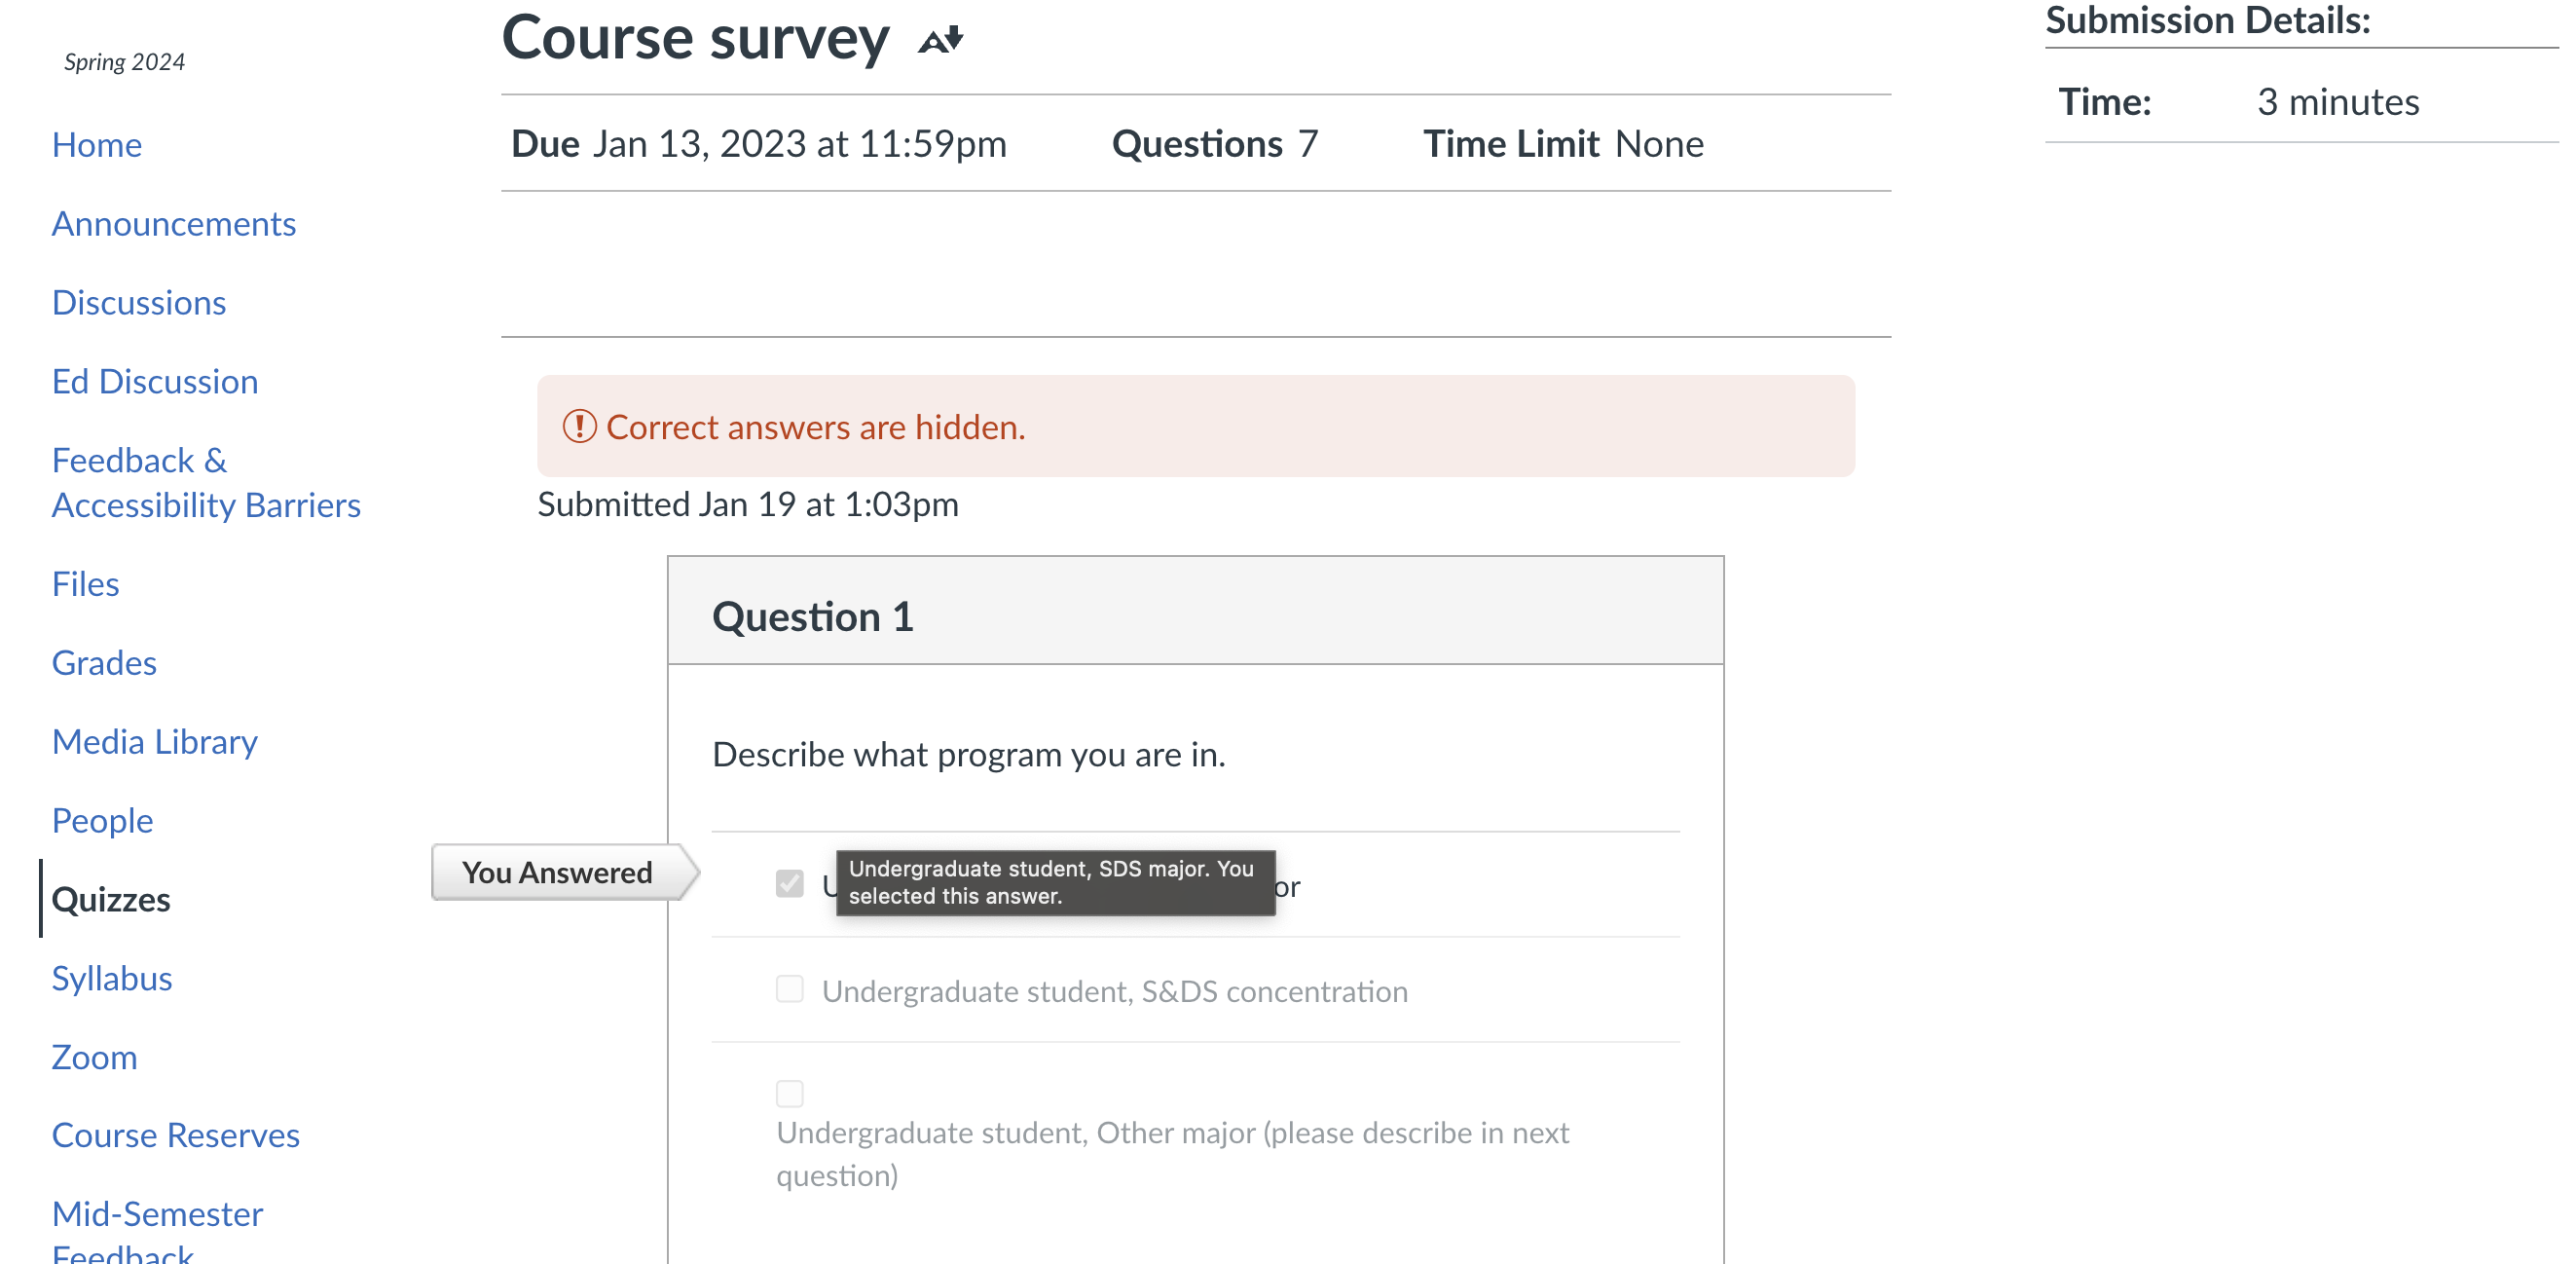
\includegraphics{img/snip of Course Survey.png}

Edit the above file name and path to show your screenshot and ensure
that it appears when you knit your document.

\paragraph{2. Download and install the latest version of
R}\label{download-and-install-the-latest-version-of-r}

See \url{https://bmacgtpm.github.io/notes/software-installation.html}
for some potentially useful tips.

The following code will show your version of R when you knit the
document. It should say \texttt{R\ version\ 4.3.2} or later. Make sure
it appears when you knit your document.

\begin{Shaded}
\begin{Highlighting}[]
\FunctionTok{R.Version}\NormalTok{()}\SpecialCharTok{$}\NormalTok{version.string}
\end{Highlighting}
\end{Shaded}

\begin{verbatim}
[1] "R version 4.3.2 (2023-10-31)"
\end{verbatim}

\paragraph{3. Download and install the latest version of
RStudio.}\label{download-and-install-the-latest-version-of-rstudio.}

See \url{https://bmacgtpm.github.io/notes/software-installation.html}
for some potentially useful tips.

This code will show your version of R when you knit the document. Make
sure it appears when you knit your document. It should say
\texttt{2023.12.0+369} (or later).

\begin{Shaded}
\begin{Highlighting}[]
\NormalTok{rstudioapi}\SpecialCharTok{::}\FunctionTok{versionInfo}\NormalTok{()}\SpecialCharTok{$}\NormalTok{long\_version}
\end{Highlighting}
\end{Shaded}

\begin{verbatim}
[1] "2023.12.0+369"
\end{verbatim}

\paragraph{4. Install/update packages}\label{installupdate-packages}

See \url{https://bmacgtpm.github.io/notes/software-installation.html}
for the packages to install.

Do not write R code for installing packages in this R Markdown. You
don't want packages to install every time you knit this document.

Check that you can load all of the libraries by running this chunk of
code and showing that it executes without error. There may be some
messages, and maybe warnings about versions. Those are ok. Make sure the
output appears when you knit the document.

\begin{Shaded}
\begin{Highlighting}[]
\FunctionTok{library}\NormalTok{(knitr)}
\FunctionTok{library}\NormalTok{(plotly)}
\FunctionTok{library}\NormalTok{(scales)}
\FunctionTok{library}\NormalTok{(DT)}
\FunctionTok{library}\NormalTok{(leaflet)}
\FunctionTok{library}\NormalTok{(gganimate)}
\FunctionTok{library}\NormalTok{(gifski)}
\FunctionTok{library}\NormalTok{(png)}
\FunctionTok{library}\NormalTok{(corrplot)}
\FunctionTok{library}\NormalTok{(GGally)}
\FunctionTok{library}\NormalTok{(ggmap)}
\FunctionTok{library}\NormalTok{(shiny)}
\FunctionTok{library}\NormalTok{(MASS)}
\FunctionTok{library}\NormalTok{(lme4)}
\FunctionTok{library}\NormalTok{(arm)}
\FunctionTok{library}\NormalTok{(pROC)}
\FunctionTok{library}\NormalTok{(MLmetrics)}
\FunctionTok{library}\NormalTok{(viridis)}
\FunctionTok{library}\NormalTok{(RSelenium)}
\FunctionTok{library}\NormalTok{(rvest)}
\FunctionTok{library}\NormalTok{(randomForest)}
\FunctionTok{library}\NormalTok{(FNN)}
\FunctionTok{library}\NormalTok{(caret)}
\FunctionTok{library}\NormalTok{(pls)}
\FunctionTok{library}\NormalTok{(devtools)}
\FunctionTok{library}\NormalTok{(splines)}
\FunctionTok{library}\NormalTok{(RecordLinkage)}
\FunctionTok{library}\NormalTok{(rsconnect)}
\FunctionTok{library}\NormalTok{(grid)}
\FunctionTok{library}\NormalTok{(foreign)}
\FunctionTok{library}\NormalTok{(maps) }\DocumentationTok{\#\# leave uncommented. For some reason GitHub Actions had a problem when this wasn\textquotesingle{}t explicitly loaded here. }

\DocumentationTok{\#\# load tidyverse last!}
\FunctionTok{library}\NormalTok{(tidyverse)}
\FunctionTok{library}\NormalTok{(pubtheme)}
\end{Highlighting}
\end{Shaded}

\paragraph{\texorpdfstring{5. Check
\texttt{gganimate}}{5. Check gganimate}}\label{check-gganimate}

See \url{https://bmacgtpm.github.io/notes/software-installation.html}.
The code from that page is below, except a custom title has been added.
Replace my name with yours, uncomment the animation code, run all of
this code.

\begin{Shaded}
\begin{Highlighting}[]
\CommentTok{\# We\textquotesingle{}ll start with a static plot}
\NormalTok{g }\OtherTok{=} \FunctionTok{ggplot}\NormalTok{(iris, }
            \FunctionTok{aes}\NormalTok{(}\AttributeTok{x =}\NormalTok{ Petal.Width, }
                \AttributeTok{y =}\NormalTok{ Petal.Length)) }\SpecialCharTok{+} 
  \FunctionTok{geom\_point}\NormalTok{() }\SpecialCharTok{+} 
  \FunctionTok{ggtitle}\NormalTok{(}\StringTok{"Nafisa Kabir\textquotesingle{}s animation"}\NormalTok{)}
\NormalTok{g}
\end{Highlighting}
\end{Shaded}

\begin{center}\includegraphics{pset00-Nafisa-Kabir_files/figure-latex/unnamed-chunk-4-1} \end{center}

\begin{Shaded}
\begin{Highlighting}[]
\CommentTok{\#a = g + }
 \CommentTok{\# transition\_states(Species,}
               \CommentTok{\#     transition\_length = 2,}
               \CommentTok{\#     state\_length = 1)}

\CommentTok{\#a  \#\# check that the animation works}

\DocumentationTok{\#\# save the animation}
\CommentTok{\#anim\_save(a, }
      \CommentTok{\#    filename = \textquotesingle{}img/test animation.gif\textquotesingle{})}
\end{Highlighting}
\end{Shaded}

There should be a static plot and an animated plot above. If the
\texttt{anim\_save} worked properly there should be a new
\texttt{test.gif} in the \texttt{img} folder that has your name. Take a
screen shot of your animated gif when the points are near the upper
right and show the screenshot here:

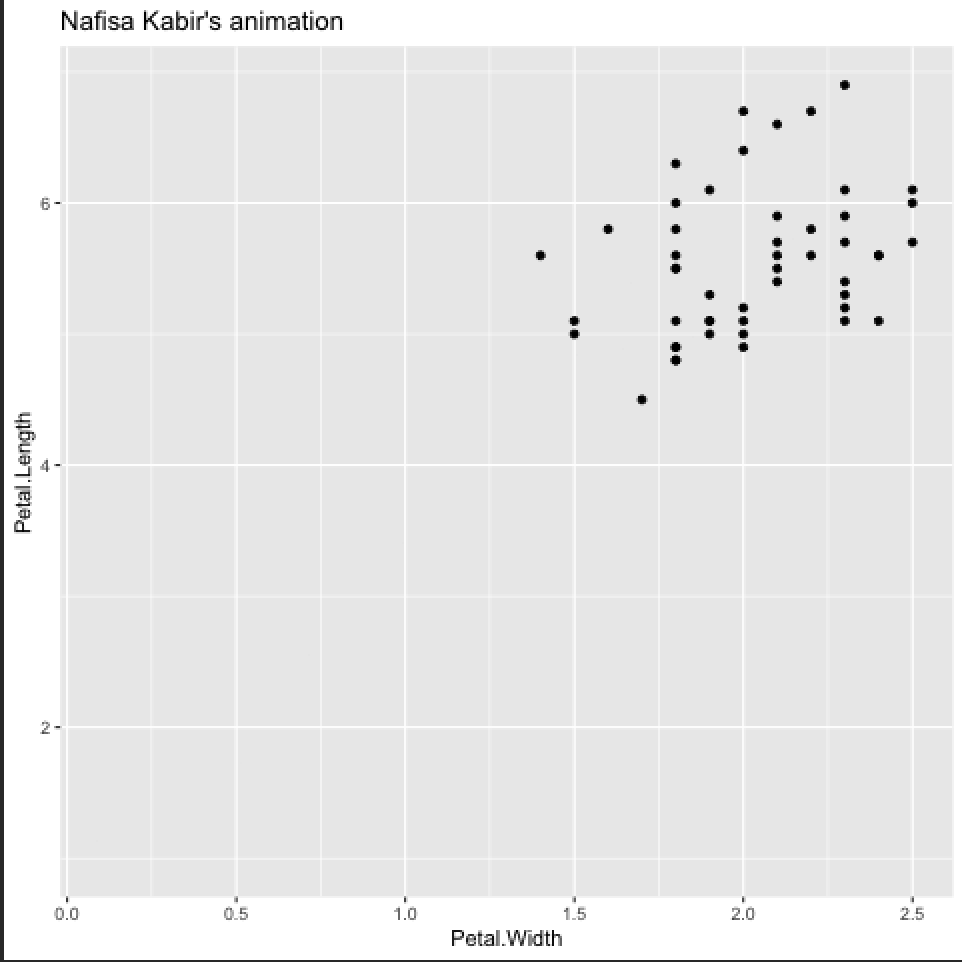
\includegraphics{img/snip of test animation.png}

If all of that works, \texttt{gganimate} is good to go! If that doesn't
work, see the tips at
\url{https://bmacgtpm.github.io/notes/software-installation.html}.

Once you have created the animation, comment out the code that creates
the animation (as I have done above). This document won't knit to PDF
with the animation code in it. You can only knit to HTML.

\paragraph{6. Bookmarks}\label{bookmarks}

See \url{https://bmacgtpm.github.io/notes/software-installation.html}.

\subsection{Part 2: Github}\label{part-2-github}

\paragraph{\texorpdfstring{7. Create a GitHub account at
\url{https://github.com/} if you don't have one. Submit your GitHub
username in Quizzes -\textgreater{} Course Survey on
Canvas.}{7. Create a GitHub account at https://github.com/ if you don't have one. Submit your GitHub username in Quizzes -\textgreater{} Course Survey on Canvas.}}\label{create-a-github-account-at-httpsgithub.com-if-you-dont-have-one.-submit-your-github-username-in-quizzes---course-survey-on-canvas.}

\paragraph{\texorpdfstring{8. Download GitHub Desktop at
\url{https://desktop.github.com/}.}{8. Download GitHub Desktop at https://desktop.github.com/.}}\label{download-github-desktop-at-httpsdesktop.github.com.}

Take a screenshot showing Github Desktop (or different software, or the
command line) and show it here.

\includegraphics{img/snip of GitHub Desktop.png}

If you have experience with Git/Github, and prefer to use different
software or the command line, that's fine, but we may not be able to
help if you have a problem.

\paragraph{\texorpdfstring{9. Clone the repo
\url{https://github.com/bmacGTPM/361-Spring-2024} and create PR as
follows.}{9. Clone the repo https://github.com/bmacGTPM/361-Spring-2024 and create PR as follows.}}\label{clone-the-repo-httpsgithub.combmacgtpm361-spring-2024-and-create-pr-as-follows.}

Clone the repo, create a new branch and name the branch
\texttt{Firstname\ Lastname} your first and last name. Make an edit to
the R Markdown file
\texttt{pset00-GitHub-pull-request-Firstname-Lastname.Rmd} to have your
name at the top instead of mine. Commit that to your branch, push those
commits to GitHub, and create a pull-request to the \texttt{main} branch
on the 361-Spring-2024 repo. Make the title of the pull request your
first and last name. For help getting started, see
\url{https://docs.github.com/en/desktop/installing-and-configuring-github-desktop/overview/getting-started-with-github-desktop}.

If you find yourself getting many notification, you can go to
\url{https://github.com/watching} to choose what notifications you get.
\href{https://docs.github.com/en/account-and-profile/managing-subscriptions-and-notifications-on-github/managing-subscriptions-for-activity-on-github/managing-your-subscriptions}{This
page} has some more info on notifications/subscriptions.

\paragraph{10. Set up Github Copilot in
RStudio}\label{set-up-github-copilot-in-rstudio}

See
\url{https://bmacgtpm.github.io/notes/github-copilot-in-rstudio.html}.

\includegraphics{img/snip of GitHub Copilot.png}

If you use Github Copilot elsewhere, take a screenshot of whatever
software you use.

\end{document}
